% Conceptual AI-generated representations; explanations remain native TeX.
\begin{frame}{Fusion Strategies}
  \SlideBody{%
    \centering
    {\fontsize{12}{14}\selectfont\bfseries\color{MoverDetailBlue}
      \makebox[4.4cm]{Early Fusion}%
      \makebox[4.4cm]{Intermediate Fusion}%
      \makebox[4.4cm]{Late Fusion}\par}
    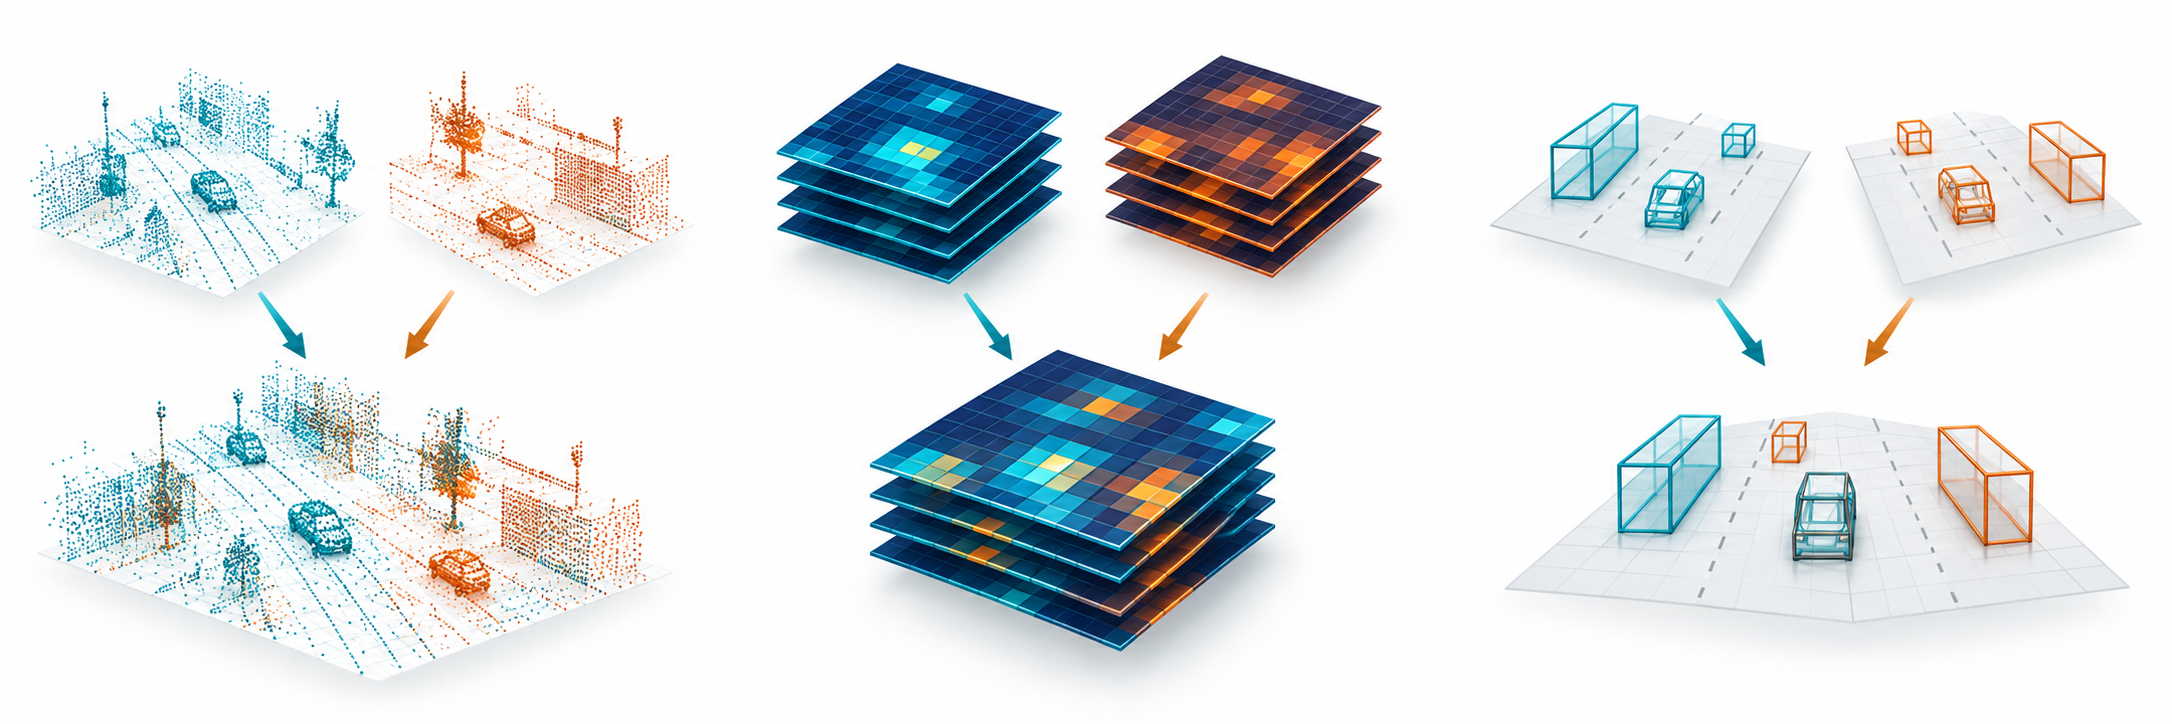
\includegraphics[width=13.2cm]{assets/illustrations/fusion-strategies.png}\par
    {\fontsize{10.5}{13}\selectfont
      \makebox[4.4cm]{\textbf{Raw LiDAR Points}}%
      \makebox[4.4cm]{\textbf{Learned Features}}%
      \makebox[4.4cm]{\textbf{Boxes, Classes, Scores}}\par
      \vspace{0.08cm}
      % Draw after the bitmap so the full divider remains visible.
      \makebox[0pt][l]{\hspace*{4.4cm}\raisebox{-0.04cm}[0pt][0pt]{\textcolor{MoverDetailBlue!40}{\rule{0.60pt}{5.62cm}}}}%
      \makebox[0pt][l]{\hspace*{8.8cm}\raisebox{-0.04cm}[0pt][0pt]{\textcolor{MoverDetailBlue!40}{\rule{0.60pt}{5.62cm}}}}%
      \makebox[4.4cm]{Fuse points, then detect}%
      \makebox[4.4cm]{Encode → Fuse → Detect}%
      \makebox[4.4cm]{Detect locally, then fuse}\par}
  }
  \SlideSource{AI-generated illustration.}
\end{frame}
